\section{The spin-zero superfluid on the combined manifolds}
\label{sec:superfluid}

\subsection{The field of the four-dimensional world}

On the combined manifold in its internal reading the 16-component field does not depend on
$x0,x5,x6,x7$. On $7+1$ the Dirac equation $(i\gamma^A_{1671}\partial_A-m_{1671})\psi_{1671}=0$, multiplied
by $\gamma^4_{1671}$ (whose square is $\mathsf 1_{16}$), becomes $i\partial_4\psi_{1671}=\sum_j\gamma^4_{1671}
\gamma^j_{1671}(-i\partial_j)\psi_{1671}+\gamma^4_{1671}m_{1671}\psi_{1671}$. On $4+4$ the Dirac equation
$(\gamma^A_{1644}\partial_A-m_{1644})\psi_{1644}=0$, multiplied by $-i\gamma^4_{1644}$ (with
$(\gamma^4_{1644})^2=-\mathsf 1_{16}$), becomes $i\partial_4\psi_{1644}=\sum_j(-\gamma^4_{1644}\gamma^j_{1644})
(-i\partial_j)\psi_{1644}+(-i\gamma^4_{1644})m_{1644}\psi_{1644}$. In both cases, for a plane wave of
momentum $\vec q=(q^1,q^2,q^3)$ in ordinary space,
\begin{align}
i\partial_4\psi_{\rm NG}&=\mathsf h_{\rm NG}(\vec q)\psi_{\rm NG},\nonumber\\
\mathsf h_{\rm NG}(\vec q)&=\sum_j\alpha^j_{\rm NG}q^j+\beta_{\rm NG}m_{\rm NG},
\label{eq:h4d}
\end{align}
with $\alpha^j_{1671}=\gamma^4_{1671}\gamma^j_{1671}$, $\beta_{1671}=\gamma^4_{1671}$ on $7+1$ and
$\alpha^j_{1644}=-\gamma^4_{1644}\gamma^j_{1644}$, $\beta_{1644}=-i\gamma^4_{1644}$ on $4+4$ (the matrices
of the project, here with $j=1,2,3$ only). They are Hermitian, square to $\mathsf 1_{16}$ and anticommute
pairwise (check P-1), so $\mathsf h_{\rm NG}(\vec q)$ has the eigenvalues $\pm\varepsilon_{\rm NG}$,
$\varepsilon_{\rm NG}=(q^2+m^2_{\rm NG})^{1/2}$ with $q=\lvert\vec q\rvert$, eight times each: the 16
components describe four four-dimensional Dirac particles, the four states of the fibre spinor
(Sec.~\ref{sec:combined}). On $7+1$ the matrices $\alpha^j_{1671}$ and $\beta_{1671}$ are real and
symmetric; on $4+4$ the $\alpha^j_{1644}$ are real and symmetric and $\beta_{1644}$ is imaginary and
antisymmetric.

\subsection{Spin-zero pairs of a single field}

For anticommuting components a pair $\psi^T_{\rm NG}\mathsf K_{\rm NG}\psi_{\rm NG}$ (with a $16\times16$ matrix
$\mathsf K_{\rm NG}$) vanishes unless $\mathsf K_{\rm NG}$ is antisymmetric. Under a Lorentz transformation
$\psi_{\rm NG}\to\exp(\varphi_{\rm NG}\Sigma^{AB}_{\rm NG})\psi_{\rm NG}$ the pair is unchanged when
$(\Sigma^{AB}_{\rm NG})^T\mathsf K_{\rm NG}+\mathsf K_{\rm NG}\Sigma^{AB}_{\rm NG}=0$. For
$\mathsf K_{\rm NG}=C^\pm_{\rm NG}\gamma^K_{\rm NG}$ the relation $C^\pm_{\rm NG}\Sigma^{AB}_{\rm NG}
(C^\pm_{\rm NG})^{-1}=-(\Sigma^{AB}_{\rm NG})^T$, which follows from $C^\pm_{\rm NG}\gamma^A_{\rm NG}
(C^\pm_{\rm NG})^{-1}=\pm(\gamma^A_{\rm NG})^T$ on $7+1$ and $\mp(\gamma^A_{\rm NG})^T$ on $4+4$, turns this
condition into $[\gamma^K_{\rm NG},\Sigma^{AB}_{\rm NG}]=0$. In eight dimensions only $K=\emptyset$ and
$K=\{0,\dots,7\}$ satisfy it for all 28 generators, and the corresponding matrices $C^\pm_{\rm NG}$ and
$C^\pm_{\rm NG}\omega_{\rm NG}$ (which equal $C^\mp_{\rm NG}$ up to sign; check K-4a) are all symmetric:

\emph{Theorem 4.} On either spacetime a single 16-component field has no pair that is a scalar of the
eight-dimensional Lorentz group.

On the combined manifold the pair need only be a scalar of the Lorentz group of the world, i.e.\
$\gamma^K_{\rm NG}$ must commute with the six $\Sigma^{AB}_{\rm NG}$ with $A,B\in\{1,2,3,4\}$; this holds when
$K$ lies in the fibre (or contains all four world indices, which gives the same matrices up to sign).
The program examines all 512 matrices $C^\pm_{\rm NG}\gamma^K_{\rm NG}$ on both spacetimes (the two
families contain the same 256 matrices up to sign; check K-4a) and records whether each is
antisymmetric, whether its pair survives for two particles at rest, and whether it is isotropic. A pair
survives at rest (it is an \emph{s-wave} pair) when it has a nonzero component on the states of positive
energy at rest, the eigenvectors of $\beta_{\rm NG}$ with eigenvalue $+1$; this is the case when
$\mathsf K_{\rm NG}$ commutes with $\gamma^4_{\rm NG}$ on $7+1$, where $\beta_{1671}$ is symmetric, and when
it anticommutes with it on $4+4$, where $\beta_{1644}$ is antisymmetric. A pair is \emph{isotropic} when it
is s-wave and $\mathsf K_{\rm NG}$ anticommutes with all three $\alpha^j_{\rm NG}$; Theorem~5 below shows that
such a pair gives a gap that does not depend on the direction of motion. Figure~\ref{fig:channels} shows
the result: on both spacetimes the nonzero, four-dimensionally scalar, s-wave, isotropic pairs are
exactly
\begin{equation}
\mathsf K^a_{\rm NG}=C^-_{\rm NG}\gamma^a_{\rm NG}\ \ (4),\qquad \mathsf K^{ab}_{\rm NG}=C^+_{\rm NG}\gamma^a_{\rm NG}\gamma^b_{\rm NG}\ \ (6),
\label{eq:channels}
\end{equation}
a vector and a two-form of the fibre (check K-4). The pairs $\psi^T_{1671}\mathsf K^a_{\rm NG}\psi_{1671}$ are
the fibre components $\Delta^a_{1671}$ of the eight-dimensional vector pair operators $\Delta^A_{1671}=
\psi^T_{1671}C^-_{1671}\gamma^A_{1671}\psi_{1671}$ of the project, and $\psi^T_{1671}\mathsf K^{ab}_{\rm NG}
\psi_{1671}$ are the fibre components $\Delta^{ab}_{1671}$ of its two-form pair operators
$\Delta^{AB}_{1671}=\psi^T_{1671}C^+_{1671}\gamma^A_{1671}\gamma^B_{1671}\psi_{1671}$; on $4+4$ the vector
pairs are the fibre components $\Delta^a_{1644}$ of $\Delta^A_{1644}=\psi^T_{1644}C^-_{1644}\gamma^A_{1644}
\psi_{1644}$, and the two-form pairs are $\Xi^{ab}_{\rm NG}=\psi^T_{1644}C^+_{1644}\gamma^a_{1644}
\gamma^b_{1644}\psi_{1644}$. The space components $C^-_{\rm NG}\gamma^j_{\rm NG}$ give s-wave pairs of spin
one, which are not isotropic. \emph{A single field, which cannot form a spin-zero pair on the
eight-dimensional spacetime, forms spin-zero pairs on the combined manifold, and these pairs carry an
index of the eight-dimensional Lorentz group.} A pair that is also a singlet of the fibre needs two
fields: with $\psi^1_{\rm NG}$, $\psi^2_{\rm NG}$ two copies of $\psi_{1671}$, the pair $\Phi^{\rm D}_{\rm NG}=
2(\psi^1_{\rm NG})^TC^+_{1671}\psi^2_{\rm NG}$ is nonzero, because the symmetric matrix $C^+_{1671}$ is allowed
between two different fields (the \emph{doublet} channel).

\begin{figure*}[t]
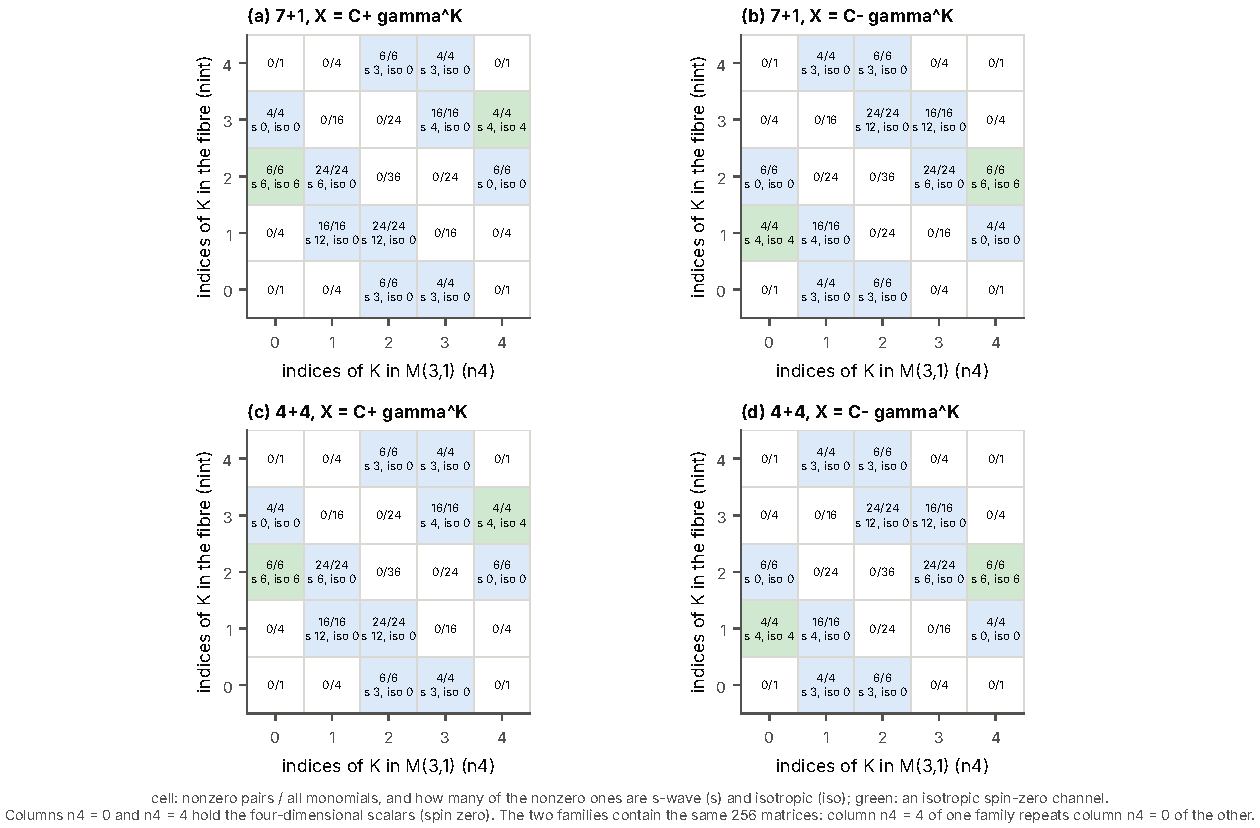
\includegraphics[width=0.85\textwidth]{../figures/fig_ng_channels.pdf}
\caption{All 512 one-field pair matrices $C^\pm_{\rm NG}\gamma^K_{\rm NG}$ on $7+1$ (a, b) and $4+4$ (c, d),
sorted by the number of indices of $K$ in the world (horizontal) and in the fibre (vertical). Each cell
gives the number of nonzero pairs among all products, and of these the numbers that are s-wave and
isotropic. Green: the isotropic spin-zero channels, Eq.~(\ref{eq:channels}). Data:
\texttt{data/ng\_pair\_channels.csv}.}
\label{fig:channels}
\end{figure*}

\subsection{The model}

We take the eight-dimensionally Lorentz-invariant interaction of the vector pairs,
\begin{equation}
\mathcal H^{\rm V}_{\rm NG}=\frac{G_{\rm NG}}4\sum_{A,B}\eta^{AB}_{1671}\,(\Delta^A_{1671})^\dagger\Delta^B_{1671}
\label{eq:hv}
\end{equation}
on $7+1$ (and the same with the tag 1644 on $4+4$), with a coupling $G_{\rm NG}>0$ of dimension
mass$^{-2}$ in the four-dimensional world, and restrict it to the fields of the world. On $7+1$ the
entries $\eta^{aa}_{1671}=\eta^{jj}_{1671}=-1$ make it attractive in the four spin-zero components
$\Delta^a_{1671}$ and in the three spin-one components $\Delta^j_{1671}$, all with the \emph{same}
coupling, and repulsive in the time component $\Delta^4_{1671}$. On $4+4$ it is attractive where
$\eta^{AA}_{1644}=-1$: in the spin-zero components $\Delta^t_{1644}$ ($t=5,6,7$) and in the time
component, which is not s-wave; it repels $\Delta^0_{1644}$ and the space components (check P-11). In
the attractive spin-zero channel the interaction is
\begin{equation}
\mathcal H^{\rm int}_{\rm NG}=-\frac{G_{\rm NG}}4\sum_a(\psi^T_{\rm NG}\mathsf K^a_{\rm NG}\psi_{\rm NG})^\dagger
(\psi^T_{\rm NG}\mathsf K^a_{\rm NG}\psi_{\rm NG})
\label{eq:hint}
\end{equation}
(on $4+4$ the sum runs over $t=5,6,7$ only). The same form with $\mathsf K^{ab}_{\rm NG}$ describes the
two-form channel, and $\mathcal H^{\rm D}_{\rm NG}=-\tfrac14G^{\rm D}_{\rm NG}(\Phi^{\rm D}_{\rm NG})^\dagger
\Phi^{\rm D}_{\rm NG}$, with its own coupling $G^{\rm D}_{\rm NG}$, the doublet channel. The mean-field
approximation replaces the product of two pairs by the products of each with the expectation value of
the other. With the pair amplitudes $\Delta^a_{\rm NG}=\tfrac12G_{\rm NG}\langle\psi^T_{\rm NG}
\mathsf K^a_{\rm NG}\psi_{\rm NG}\rangle$ (complex numbers),
\begin{align}
\mathcal H^{\rm MF}_{\rm NG}&=\psi^\dagger_{\rm NG}(\mathsf h_{\rm NG}-\mu_{\rm NG})\psi_{\rm NG}+\frac{\lvert\Delta_{\rm NG}\rvert^2}{G_{\rm NG}}\nonumber\\
&\quad-\tfrac12\sum_a\big(\Delta^{a*}_{\rm NG}\,\psi^T_{\rm NG}\mathsf K^a_{\rm NG}\psi_{\rm NG}+{\rm h.c.}\big),
\label{eq:hmf}
\end{align}
with $\lvert\Delta_{\rm NG}\rvert^2=\sum_a\lvert\Delta^a_{\rm NG}\rvert^2$ and the chemical potential
$\mu_{\rm NG}$ that fixes the density of fermions. The two-form amplitudes $\Delta^{ab}_{\rm NG}$ and the
doublet amplitude $\Delta^{\rm D}_{\rm NG}=\tfrac12G^{\rm D}_{\rm NG}\langle\Phi^{\rm D}_{\rm NG}\rangle$ are
defined in the same way.

\subsection{Bogoliubov-de Gennes spectrum}

With the Nambu spinor $\mathcal N_{\rm NG}(\vec q)=(\psi_{\rm NG}(\vec q),\psi_{\rm NG}(-\vec q)^{\dagger T})$ of
32 components, $\sum_{\vec q}\mathcal H^{\rm MF}_{\rm NG}=\tfrac12\sum_{\vec q}\mathcal N^\dagger_{\rm NG}
\mathsf H_{\rm NG}(\vec q)\mathcal N_{\rm NG}+\text{constant}$, with the Bogoliubov-de Gennes matrix
\begin{align}
\mathsf H_{\rm NG}(\vec q)&=\begin{pmatrix}\mathsf h_{\rm NG}(\vec q)-\mu_{\rm NG}&\mathsf P_{\rm NG}\\
\mathsf P_{\rm NG}^\dagger&-(\mathsf h_{\rm NG}(-\vec q)-\mu_{\rm NG})^T\end{pmatrix},\nonumber\\
\mathsf P_{\rm NG}&=-\sum_a\Delta^a_{\rm NG}(\mathsf K^a_{\rm NG})^\dagger.
\label{eq:bdg}
\end{align}
For the doublet the Nambu spinor is $(\psi^1_{\rm NG}(\vec q),\psi^2_{\rm NG}(-\vec q)^{\dagger T})$, the factor
$\tfrac12$ is absent, and $\mathsf P_{\rm NG}=\Delta^{\rm D}_{\rm NG}(C^+_{1671})^*$. The lower right block equals
$\mu_{\rm NG}-\beta_{1671}\mathsf h_{\rm NG}(\vec q)\beta_{1671}$ on $7+1$ and $\mathsf h_{\rm NG}(\vec q)+
\mu_{\rm NG}$ on $4+4$, by the symmetry properties of $\alpha^j_{\rm NG}$ and $\beta_{\rm NG}$ stated above.
The grand potential per volume at zero temperature, the \emph{effective potential} of the superfluid,
is the ground-state energy of $\mathcal H^{\rm MF}_{\rm NG}$ per volume:
\begin{equation}
\Omega_{\rm NG}=\frac{\lvert\Delta_{\rm NG}\rvert^2}{G_{\rm NG}}-\frac12\int\frac{d^3q}{(2\pi)^3}
\sum_{\mathcal E_{\rm NG}>0}\mathcal E_{\rm NG}(\vec q),
\label{eq:omega}
\end{equation}
summed over the positive eigenvalues $\mathcal E_{\rm NG}$ of $\mathsf H_{\rm NG}(\vec q)$, up to terms that do not
depend on the pair amplitudes. The factor $\tfrac12$ appears because each mode of one field occurs twice in
the Nambu spinor; for the doublet, whose Nambu spinor contains each mode once, it is absent (and
$G^{\rm D}_{\rm NG}$ replaces $G_{\rm NG}$).

\emph{Theorem 5 (isotropic gap).} Let $\mathsf P_{\rm NG}$ commute with $\beta_{\rm NG}$ (on $7+1$) or
anticommute with it (on $4+4$), anticommute with every $\alpha^j_{\rm NG}$, and satisfy
$\mathsf P_{\rm NG}\mathsf P_{\rm NG}^\dagger=\mathsf P^\dagger_{\rm NG}\mathsf P_{\rm NG}=\lvert\Delta_{\rm NG}\rvert^2\mathsf 1_{16}$.
Then the eigenvalues of $\mathsf H_{\rm NG}(\vec q)$ are $\pm E^+_{\rm NG}$ and $\pm E^-_{\rm NG}$, eight times
each, with
\begin{equation}
E^\pm_{\rm NG}=\big[(\varepsilon_{\rm NG}\pm\mu_{\rm NG})^2+\lvert\Delta_{\rm NG}\rvert^2\big]^{1/2}.
\label{eq:epm}
\end{equation}
\emph{Proof} (for $7+1$; on $4+4$ replace $\mu_{\rm NG}-\beta_{1671}\mathsf h_{\rm NG}\beta_{1671}$ by
$\mathsf h_{\rm NG}+\mu_{\rm NG}$ and use the anticommutation with $\beta_{1644}$). The off-diagonal block of
$\mathsf H_{\rm NG}^2$ is $(\mathsf h_{\rm NG}-\mu_{\rm NG})\mathsf P_{\rm NG}+\mathsf P_{\rm NG}(\mu_{\rm NG}-
\beta_{1671}\mathsf h_{\rm NG}\beta_{1671})=\mathsf h_{\rm NG}\mathsf P_{\rm NG}-\mathsf P_{\rm NG}\beta_{1671}
\mathsf h_{\rm NG}\beta_{1671}$; since $\beta_{1671}\mathsf h_{\rm NG}(\vec q)\beta_{1671}=-\sum_j\alpha^j_{1671}q^j+
\beta_{1671}m_{1671}$ and $\mathsf P_{\rm NG}$ anticommutes with the $\alpha^j_{1671}$ and commutes with
$\beta_{1671}$, $\mathsf P_{\rm NG}\beta_{1671}\mathsf h_{\rm NG}\beta_{1671}=\mathsf h_{\rm NG}\mathsf P_{\rm NG}$, and the
block vanishes. The diagonal blocks are $(\mathsf h_{\rm NG}-\mu_{\rm NG})^2+\lvert\Delta_{\rm NG}\rvert^2$ and
$(\mu_{\rm NG}-\beta_{1671}\mathsf h_{\rm NG}\beta_{1671})^2+\lvert\Delta_{\rm NG}\rvert^2$, each with the
eigenvalues $(\varepsilon_{\rm NG}+\mu_{\rm NG})^2+\lvert\Delta_{\rm NG}\rvert^2$ and $(\varepsilon_{\rm NG}-
\mu_{\rm NG})^2+\lvert\Delta_{\rm NG}\rvert^2$, eight times each. Hence $\mathsf H_{\rm NG}$ has the eigenvalues
$\pm E^+_{\rm NG}$, $\pm E^-_{\rm NG}$ with 16 eigenvalues of each modulus. $\mathsf H_{\rm NG}$ is traceless
(its diagonal blocks have the traces $\mathrm{tr}\,\mathsf h_{\rm NG}(\vec q)=0$ and
$-\mathrm{tr}\,\mathsf h_{\rm NG}(-\vec q)=0$, apart from $\mp16\mu_{\rm NG}$, which cancel). When
$E^+_{\rm NG}/E^-_{\rm NG}$ is irrational, a vanishing sum of the eigenvalues requires as many eigenvalues
$+E^\pm_{\rm NG}$ as $-E^\pm_{\rm NG}$, i.e.\ eight of each; the eigenvalues depend continuously on
$\mu_{\rm NG}$ and never pass through zero (they have moduli $E^\pm_{\rm NG}\ge\lvert\Delta_{\rm NG}\rvert>0$),
so the multiplicities are eight for all parameters. $\square$

The channels of Eq.~(\ref{eq:channels}) satisfy the hypotheses for every real direction of the pair
amplitudes (and every common phase): for real amplitudes the cross terms $\Delta^a_{\rm NG}\Delta^b_{\rm NG}$
of $\mathsf P_{\rm NG}\mathsf P_{\rm NG}^\dagger$ multiply the antisymmetric combinations $\gamma^a_{\rm NG}
\gamma^b_{\rm NG}+\gamma^b_{\rm NG}\gamma^a_{\rm NG}=0$ ($a\ne b$). The program confirms the spectrum on random
momenta, chemical potentials, masses and directions for the vector, two-form and doublet channels on
both spacetimes (check P-2). With Eq.~(\ref{eq:omega}) every isotropic state has
\begin{align}
\Omega_{\rm NG}&=\frac{\lvert\Delta_{\rm NG}\rvert^2}{G_{\rm NG}}-\nu_{\rm NG}\int\frac{d^3q}{(2\pi)^3}
\big(E^+_{\rm NG}+E^-_{\rm NG}\big),\nonumber\\
\frac1{G_{\rm NG}}&=\frac{\nu_{\rm NG}}2\int\frac{d^3q}{(2\pi)^3}
\Big(\frac1{E^+_{\rm NG}}+\frac1{E^-_{\rm NG}}\Big),
\label{eq:gap}
\end{align}
the second equation (the \emph{gap equation}) being the condition for a minimum away from zero, with
$\nu_{\rm NG}=4$ for one field and $\nu_{\rm NG}=8$ for the doublet (for which $G^{\rm D}_{\rm NG}$ replaces
$G_{\rm NG}$): eight positive eigenvalues of each kind, times $\tfrac12$ or 1. The program verifies the
first equation against the numerical sum over the eigenvalues of $\mathsf H_{\rm NG}$ (check P-5).
Throughout, the momentum integrals are cut off at $\lvert\vec q\rvert=\Lambda_{\rm NG}$, and we set
$\Lambda_{\rm NG}=1$.

\emph{Non-unitary and spin-one states.} For the complex direction $\Delta^0_{\rm NG}=\lvert\Delta_{\rm NG}
\rvert\cos\upsilon_{\rm NG}$, $\Delta^5_{\rm NG}=i\lvert\Delta_{\rm NG}\rvert\sin\upsilon_{\rm NG}$,
$\Delta^6_{\rm NG}=\Delta^7_{\rm NG}=0$ of the vector amplitudes on $7+1$, with an angle $\upsilon_{\rm NG}$,
the cross terms no longer cancel. With $C^-_{1671}$ orthogonal and the $\gamma^a_{1671}$ real,
antisymmetric and of square $-\mathsf 1_{16}$, $(\mathsf K^a_{\rm NG})^\dagger\mathsf K^b_{\rm NG}=
-\gamma^a_{1671}\gamma^b_{1671}$, and one finds
$\mathsf P_{\rm NG}\mathsf P^\dagger_{\rm NG}=\lvert\Delta_{\rm NG}\rvert^2(\mathsf 1_{16}+\sin2\upsilon_{\rm NG}\,
i\gamma^0_{1671}\gamma^5_{1671})$ and $\mathsf P^\dagger_{\rm NG}\mathsf P_{\rm NG}=\lvert\Delta_{\rm NG}\rvert^2(\mathsf 1_{16}-
\sin2\upsilon_{\rm NG}\,i\gamma^0_{1671}\gamma^5_{1671})$, where $i\gamma^0_{1671}\gamma^5_{1671}$ is
Hermitian, has square $\mathsf 1_{16}$, and commutes with $\alpha^j_{1671}$ and $\beta_{1671}$. The
off-diagonal block of $\mathsf H_{\rm NG}^2$ still vanishes, and on the eigenspaces of $i\gamma^0_{1671}\gamma^5_{1671}$ the
gap splits into $\lvert\Delta_{\rm NG}\rvert(1\pm\zeta_{\rm NG})^{1/2}$, $\zeta_{\rm NG}=\lvert\sin
2\upsilon_{\rm NG}\rvert$, still independent of the direction of motion (check P-3a, which also confirms
the multiplicities, four each); the \emph{chiral} state $\upsilon_{\rm NG}=\pi/4$ has the gaps
$\sqrt2\lvert\Delta_{\rm NG}\rvert$ and 0. The spin-one pair $C^-_{\rm NG}\gamma^1_{\rm NG}$ (direction
$\hat n_{\rm NG}$ along $x1$) commutes with $\alpha^1_{\rm NG}$ instead of anticommuting with it, and its
spectrum is (check P-4)
\begin{align}
(E^{(1)\pm}_{\rm NG})^2&=\varepsilon_{\rm NG}^2+\mu_{\rm NG}^2+\lvert\Delta_{\rm NG}\rvert^2\nonumber\\
&\quad\pm2\big[\mu_{\rm NG}^2\varepsilon_{\rm NG}^2+\lvert\Delta_{\rm NG}\rvert^2(q^1)^2\big]^{1/2},
\label{eq:spin1}
\end{align}
eight times each, which depends on the angle between $\vec q$ and $\hat n_{\rm NG}$. For $\vec q$ along
$\hat n_{\rm NG}$ on the Fermi surface $\varepsilon_{\rm NG}=\mu_{\rm NG}$, the lower energy is
$\lvert\Delta_{\rm NG}\rvert m_{\rm NG}/\mu_{\rm NG}$ to leading order in $\lvert\Delta_{\rm NG}\rvert$; for
massless fermions $(E^{(1)-}_{\rm NG})^2=(q-(\mu_{\rm NG}^2+\lvert\Delta_{\rm NG}\rvert^2)^{1/2})^2$ along
$\hat n_{\rm NG}$, which vanishes exactly at $q=(\mu_{\rm NG}^2+\lvert\Delta_{\rm NG}\rvert^2)^{1/2}$.

\subsection{Vacuum and finite density}

\emph{Vacuum.} At $\mu_{\rm NG}=0$ a pair condensate forms only if the gap equation~(\ref{eq:gap}) has a
solution, i.e.\ above the critical coupling $G^{\rm crit}_{\rm NG}$ with $1/G^{\rm crit}_{\rm NG}=\nu_{\rm NG}
\int d^3q\,(2\pi)^{-3}\varepsilon_{\rm NG}^{-1}$ (the right side of the gap equation at
$\lvert\Delta_{\rm NG}\rvert\to0$, which is its largest value); for massless fermions $\int d^3q\,
(2\pi)^{-3}q^{-1}=\Lambda_{\rm NG}^2/(4\pi^2)$ and $G^{\rm crit}_{\rm NG}=4\pi^2/(\nu_{\rm NG}
\Lambda_{\rm NG}^2)$: $\pi^2/\Lambda_{\rm NG}^2$ for one field and $\pi^2/(2\Lambda_{\rm NG}^2)$ for the doublet
(the program finds {{GEN:gcrit_one}} and {{GEN:gcrit_doublet}}; for $m_{\rm NG}=0.2$ the one-field value
is {{GEN:gcrit_one_m02}}; check P-6, Fig.~\ref{fig:gap}). The vacuum condensate is a four-dimensional
Lorentz scalar, so the vacuum of the world stays Lorentz invariant.

\begin{figure}[t]
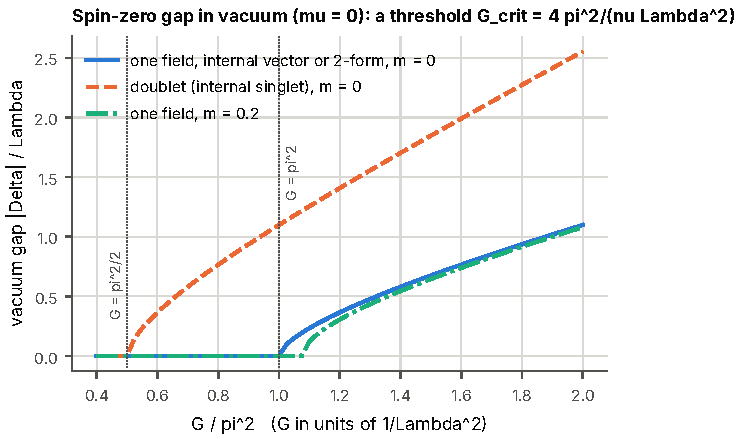
\includegraphics[width=\columnwidth]{../figures/fig_ng_gap.pdf}
\caption{Gap of the vacuum versus coupling. A single field condenses in the internal-vector or
two-form channel above $G_{\rm NG}=\pi^2$ ($m_{\rm NG}=0$; blue) or slightly above it ($m_{\rm NG}=0.2$;
aqua); the doublet (orange) above $\pi^2/2$. Units: $\Lambda_{\rm NG}=1$; gaps of order
$\Lambda_{\rm NG}$ and more lie outside the range in which a model with a cutoff is meaningful. Data:
\texttt{data/ng\_gap\_vs\_coupling.csv}.}
\label{fig:gap}
\end{figure}

\emph{Finite density.} For $\mu_{\rm NG}>m_{\rm NG}$ there is a Fermi surface at
$q=q^{\rm F}_{\rm NG}=(\mu_{\rm NG}^2-m_{\rm NG}^2)^{1/2}$, where $E^-_{\rm NG}$ becomes as small as
$\lvert\Delta_{\rm NG}\rvert$; the integral of $1/E^-_{\rm NG}$ then grows like $\ln(1/\lvert\Delta_{\rm NG}
\rvert)$, and the gap equation has a solution for every attraction (Cooper instability~\cite{BCS1957}).
Near the Fermi surface $d^3q/(2\pi)^3=q^2dq/(2\pi^2)$ and $q\,dq=\varepsilon_{\rm NG}d\varepsilon_{\rm NG}$
give $d^3q/(2\pi)^3\approx q^{\rm F}_{\rm NG}\mu_{\rm NG}\,d\varepsilon_{\rm NG}/(2\pi^2)$, so at weak coupling
$\ln\lvert\Delta_{\rm NG}\rvert=\text{constant}-2\pi^2/(\nu_{\rm NG}q^{\rm F}_{\rm NG}\mu_{\rm NG}G_{\rm NG})$. The
program finds a gap for a coupling that is subcritical in the vacuum, none below $\mu_{\rm NG}=m_{\rm NG}$,
and a slope of $\ln\lvert\Delta_{\rm NG}\rvert$ against $1/G_{\rm NG}$ equal to {{GEN:bcs_ratio}} times the
predicted one (check P-7, Fig.~\ref{fig:density}).

\begin{figure*}[t]
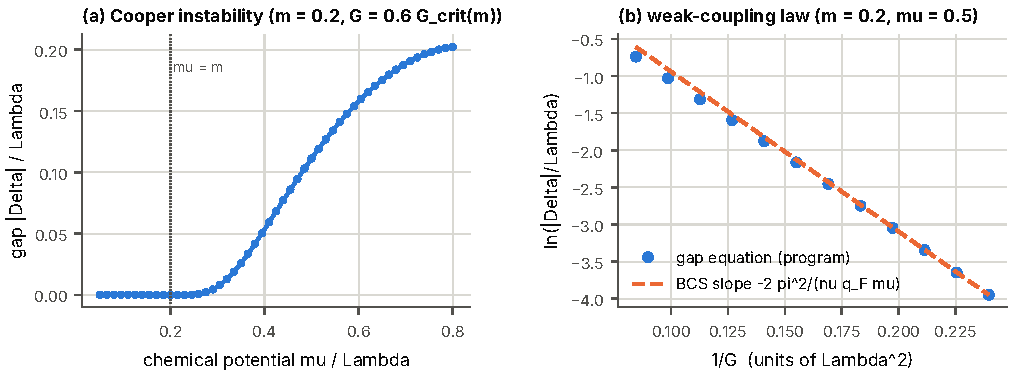
\includegraphics[width=0.92\textwidth]{../figures/fig_ng_density.pdf}
\caption{(a) The gap versus the chemical potential for a coupling below the vacuum threshold: it appears
when a Fermi surface exists. (b) At weak coupling the logarithm of the gap falls linearly in
$1/G_{\rm NG}$ with the slope $-2\pi^2/(\nu_{\rm NG}q^{\rm F}_{\rm NG}\mu_{\rm NG})$ (dashed). Data:
\texttt{data/ng\_gap\_vs\_mu.csv}, \texttt{data/ng\_bcs\_law.csv}.}
\label{fig:density}
\end{figure*}

\subsection{Which state wins}

The interaction~(\ref{eq:hv}) treats the four spin-zero and the three spin-one components of the vector
pairs on $7+1$ alike. The ground state is nevertheless the polar spin-zero state: \emph{at every
amplitude $\lvert\Delta_{\rm NG}\rvert$, $\Omega_{\rm NG}$ is lowest for the isotropic (polar) state.} For the
non-unitary states the two gaps $\lvert\Delta_{\rm NG}\rvert(1\pm\zeta_{\rm NG})^{1/2}$ have the mean square
$\lvert\Delta_{\rm NG}\rvert^2$, and the square root is concave, so with $\xi_{\rm NG}=\varepsilon_{\rm NG}\pm
\mu_{\rm NG}$, $\sum_\pm[\xi_{\rm NG}^2+\lvert\Delta_{\rm NG}\rvert^2(1\pm\zeta_{\rm NG})]^{1/2}\le
2[\xi_{\rm NG}^2+\lvert\Delta_{\rm NG}\rvert^2]^{1/2}$ at every momentum, and the subtracted integral in
Eq.~(\ref{eq:omega}) is smaller. For the spin-one state the sum of the squares of the two energies of
Eq.~(\ref{eq:spin1}) is the same as for the polar state, $2(\varepsilon_{\rm NG}^2+\mu_{\rm NG}^2+
\lvert\Delta_{\rm NG}\rvert^2)$, but the square of their product is smaller by $4\lvert\Delta_{\rm NG}\rvert^2
(q^1)^2$, so their sum $[(E^{(1)+}_{\rm NG})^2+(E^{(1)-}_{\rm NG})^2+2E^{(1)+}_{\rm NG}E^{(1)-}_{\rm NG}]^{1/2}$ is
smaller. The program confirms the order at all {{GEN:n_omega_grid}} amplitudes of its grid (check P-8,
Fig.~\ref{fig:states}): at $m_{\rm NG}=0.2$, $\mu_{\rm NG}=0.5$ and $G_{\rm NG}=0.9\,G^{\rm crit}_{\rm NG}$ (the
critical coupling for $m_{\rm NG}=0.2$) the smallest values of $\Omega_{\rm NG}$ on the grid are
{{GEN:omega_min_polar}} (polar
spin zero), {{GEN:omega_min_chiral}} (chiral) and {{GEN:omega_min_spin1}} (spin one), in units of
$10^{-3}\Lambda_{\rm NG}^4$, and the polar gap is {{GEN:gap_polar}}.

\begin{figure*}[t]
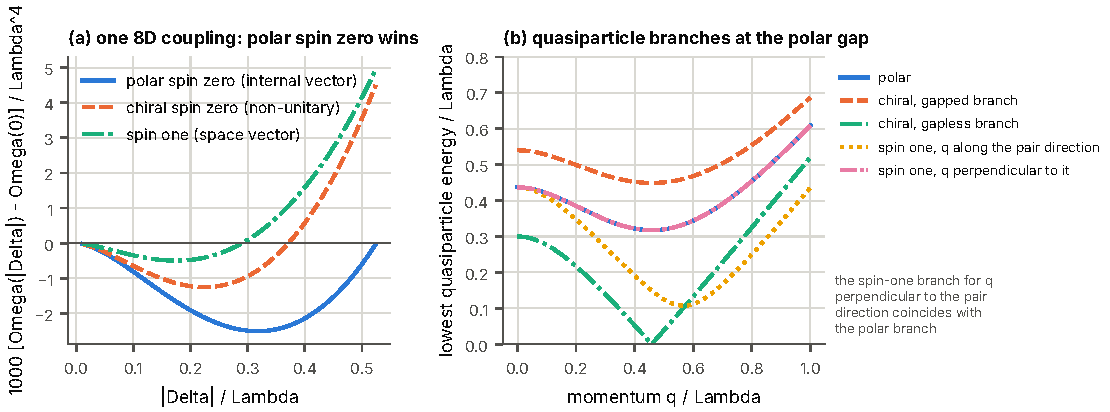
\includegraphics[width=0.92\textwidth]{../figures/fig_ng_states.pdf}
\caption{(a) Effective potential of the polar spin-zero, chiral spin-zero and spin-one states for one
eight-dimensional coupling ($m_{\rm NG}=0.2$, $\mu_{\rm NG}=0.5$, $G_{\rm NG}=0.9\,G^{\rm crit}_{\rm NG}$). (b)
Lowest quasi-particle energies at the polar gap: the polar branch, the two branches of the chiral state
(one gapless), and the spin-one branch along and perpendicular to the direction of the pair. Data:
\texttt{data/ng\_omega\_states.csv}, \texttt{data/ng\_dispersion.csv}.}
\label{fig:states}
\end{figure*}

\subsection{The amplitude mode}

By the proof of Theorem~5, each isotropic channel decomposes into independent pairs of a particle and a
hole with the $2\times2$ matrices $\big(\begin{smallmatrix}\xi_{\rm NG}&\lvert\Delta_{\rm NG}\rvert\\
\lvert\Delta_{\rm NG}\rvert&-\xi_{\rm NG}\end{smallmatrix}\big)$, $\xi_{\rm NG}=\varepsilon_{\rm NG}\pm
\mu_{\rm NG}$, as in the theory of Bardeen, Cooper and Schrieffer. Let the amplitude oscillate,
$\lvert\Delta_{\rm NG}\rvert\to\lvert\Delta_{\rm NG}\rvert+\delta_{\rm NG}\exp(-iw_{\rm NG}x4)$ with a small real
$\delta_{\rm NG}$ and a frequency $w_{\rm NG}$. In each block it couples to the off-diagonal matrix
$\big(\begin{smallmatrix}0&1\\1&0\end{smallmatrix}\big)$, whose matrix element between the two eigenstates
of energy $\pm E^\pm_{\rm NG}$ has the square $\xi_{\rm NG}^2/(E^\pm_{\rm NG})^2$; the linear response of
the pair amplitude then gives the inverse propagator of the oscillation (random-phase approximation),
\begin{align}
\Pi^{\rm A}_{\rm NG}(w_{\rm NG})&=\frac1{G_{\rm NG}}\nonumber\\
&\quad-\frac{\nu_{\rm NG}}2\int\frac{d^3q}{(2\pi)^3}\sum_\pm
\frac{4(\varepsilon_{\rm NG}\pm\mu_{\rm NG})^2}{E^\pm_{\rm NG}[4(E^\pm_{\rm NG})^2-w_{\rm NG}^2]},
\label{eq:pia}
\end{align}
a mode existing where it vanishes. Eliminating $1/G_{\rm NG}$ with the gap equation and using
$(E^\pm_{\rm NG})^2-(\varepsilon_{\rm NG}\pm\mu_{\rm NG})^2=\lvert\Delta_{\rm NG}\rvert^2$ gives
\begin{align}
\Pi^{\rm A}_{\rm NG}(w_{\rm NG})&=(4\lvert\Delta_{\rm NG}\rvert^2-w_{\rm NG}^2)\,c^\sigma_{\rm NG}(w_{\rm NG}),\nonumber\\
c^\sigma_{\rm NG}(w_{\rm NG})&=\frac{\nu_{\rm NG}}2\int\frac{d^3q}{(2\pi)^3}\sum_\pm\frac1{E^\pm_{\rm NG}
[4(E^\pm_{\rm NG})^2-w_{\rm NG}^2]},
\label{eq:csigma}
\end{align}
and $c^\sigma_{\rm NG}$ is finite and positive for $0\le w_{\rm NG}\le2\lvert\Delta_{\rm NG}\rvert$ in the
vacuum (there $E^\pm_{\rm NG}\ge\lvert\Delta_{\rm NG}\rvert$, and near the minimum the factor $q^2$ of the
volume element cancels the zero of the denominator). Hence the amplitude (Higgs) mode has the mass
$m^\sigma_{\rm NG}=2\lvert\Delta_{\rm NG}\rvert$ exactly, at the threshold for breaking a pair. The program
evaluates $c^\sigma_{\rm NG}$ on $[0,2\lvert\Delta_{\rm NG}\rvert]$ for $m_{\rm NG}=0$, $G_{\rm NG}=1.5\pi^2$, where
$\lvert\Delta_{\rm NG}\rvert=${{GEN:gap_amplitude}}, and checks the static limit: $\Pi^{\rm A}_{\rm NG}(0)$ must
equal half the second derivative of $\Omega_{\rm NG}$ with respect to $\lvert\Delta_{\rm NG}\rvert$ at the
minimum, and the two numbers are {{GEN:pia0}} and {{GEN:omega_second}} (check P-9,
Fig.~\ref{fig:amplitude}). For an oscillation of the phase, the matrix element squared is 1 instead of
$\xi_{\rm NG}^2/(E^\pm_{\rm NG})^2$, and the same steps give the inverse propagator
$-w_{\rm NG}^2\,c^\sigma_{\rm NG}(w_{\rm NG})$, which vanishes at $w_{\rm NG}=0$: the phase oscillation is a
Goldstone mode (derived here, not machine-checked).

\begin{figure}[t]
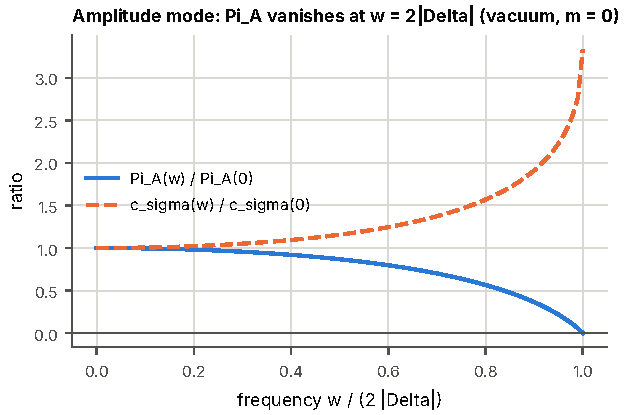
\includegraphics[width=\columnwidth]{../figures/fig_ng_amplitude.pdf}
\caption{The amplitude mode in the vacuum ($m_{\rm NG}=0$, $G_{\rm NG}=1.5\pi^2$): the inverse propagator
$\Pi^{\rm A}_{\rm NG}$ vanishes at $w_{\rm NG}=2\lvert\Delta_{\rm NG}\rvert$, where $c^\sigma_{\rm NG}$ is still
finite. Data: \texttt{data/ng\_amplitude\_mode.csv}.}
\label{fig:amplitude}
\end{figure}

\subsection{Spontaneous breaking and the locking of a Lorentz rotation to the fermion number}

On $7+1$ the one-field theory is symmetric under the Lorentz group of the world, the rotations of the
fibre and the fermion number. We denote by $\mathcal T^{ab}_{\rm NG}$ ($a<b$) the generator of rotations of
the fibre in the plane of $xa$ and $xb$; on the vector amplitudes it acts by changing $\Delta^a_{\rm NG}$ by
$-\Delta^b_{\rm NG}$ and $\Delta^b_{\rm NG}$ by $+\Delta^a_{\rm NG}$ per unit parameter (and on the two-form
amplitudes as on the products of two vectors). The fermion number $\psi_{\rm NG}\to\exp(i\varphi_{\rm NG})
\psi_{\rm NG}$ multiplies every pair by $\exp(2i\varphi_{\rm NG})$; its generator $F_{\rm NG}$ multiplies every
pair amplitude by $2i$. The condensates are scalars of the world, so its Lorentz group stays unbroken;
the symmetry of the fibre and of the fermion number, a group of dimension 7, is broken to the stabilizer
of the condensate, which the program computes exactly (check P-10, Fig.~\ref{fig:goldstone}):
\begin{itemize}
\item polar vector, only $\Delta^0_{\rm NG}\neq0$: unbroken rotations of $x5,x6,x7$ (dimension 3); four
broken generators;
\item chiral vector, $\Delta^5_{\rm NG}=i\Delta^0_{\rm NG}$ and $\Delta^6_{\rm NG}=\Delta^7_{\rm NG}=0$: unbroken
$\mathcal T^{05}_{\rm NG}+\tfrac12F_{\rm NG}$ and $\mathcal T^{67}_{\rm NG}$ (dimension 2); five broken generators;
\item self-dual two-form, $\Delta^{05}_{\rm NG}=\Delta^{67}_{\rm NG}$ and all other components zero: unbroken
$U(1)\times SU(2)$ (dimension 4); three broken generators.
\end{itemize}
For the chiral state, $\mathcal T^{05}_{\rm NG}$ changes $(\Delta^0_{\rm NG},\Delta^5_{\rm NG})=(1,i)\Delta^0_{\rm NG}$
by $(-i,1)\Delta^0_{\rm NG}=-i(1,i)\Delta^0_{\rm NG}$, and $\tfrac12F_{\rm NG}$ by $+i(1,i)\Delta^0_{\rm NG}$, so their
sum leaves it unchanged. The unbroken generator $\mathcal T^{05}_{\rm NG}+\tfrac12F_{\rm NG}$ is the sum of a
rotation in the plane of $x0$ and $x5$---an element of the eight-dimensional Lorentz group---and the
fermion number: \emph{a Lorentz rotation of eight dimensions is locked to an internal charge in the
symmetry of a four-dimensionally Lorentz-invariant vacuum.} In four dimensions this is allowed, because
the rotation of the fibre is an internal symmetry there; in eight dimensions it is possible because the
combined manifold breaks the eight-dimensional Poincar\'e group (H1). Seen in eight dimensions, a polar
vector condensate is a vector of the Lorentz group pointing into the fibre; its stabilizer in
$\mathfrak{so}(7,1)$ is $\mathfrak{so}(6,1)$, of dimension 21, and 12 of its generators mix the world with
the fibre (check K-10). (At finite density, two broken generators whose commutator has a nonzero
expectation value give one Goldstone mode with quadratic dispersion instead of two; we count broken
generators and do not analyse the dispersions.)

\begin{figure}[t]
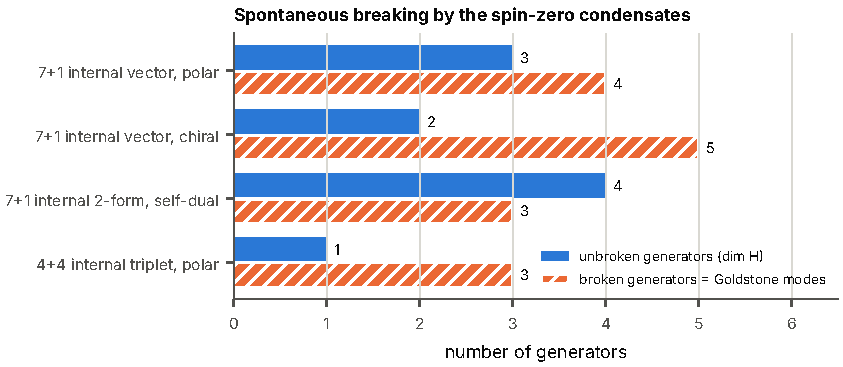
\includegraphics[width=\columnwidth]{../figures/fig_ng_goldstone.pdf}
\caption{Unbroken and broken generators of the spin-zero phases. Data: \texttt{data/ng\_goldstone.csv}.}
\label{fig:goldstone}
\end{figure}

\subsection{The superfluid on 4+4}

\emph{Theorem 6 (Wick map).} For every complex vector amplitude, the eigenvalues of the $4+4$ matrix
$\mathsf H_{\rm NG}(\vec q)$ equal those of the $7+1$ matrix with $\Delta^0_{\rm NG}$ replaced by
$i\Delta^0_{\rm NG}$; for the two-form channel, with $\Delta^{0t}_{\rm NG}$ replaced by $i\Delta^{0t}_{\rm NG}$.

\emph{Why.} For every complex amplitude $\mathsf P_{\rm NG}$ anticommutes with the $\alpha^j_{\rm NG}$ and
commutes (on $7+1$) or anticommutes (on $4+4$) with $\beta_{\rm NG}$, so, as in the proof of Theorem~5,
$\mathsf H_{\rm NG}^2$ is block diagonal; its blocks are a kinetic part with the eigenvalues
$(\varepsilon_{\rm NG}\pm\mu_{\rm NG})^2$, eight times each, plus $\mathsf P_{\rm NG}\mathsf P^\dagger_{\rm NG}$ or
$\mathsf P^\dagger_{\rm NG}\mathsf P_{\rm NG}$. These two products are combinations of $\mathsf 1_{16}$ and the
products $\gamma^a_{\rm NG}\gamma^b_{\rm NG}$ of fibre matrices, with coefficients quadratic in the
amplitudes. The products act on the fibre factor of $\mathbb C^4\otimes\mathbb C^4$ (check K-3) and commute
with the kinetic part, which acts on the world factor; the spectrum of $\mathsf H^2_{\rm NG}$ is therefore
fixed by the algebraic relations and the Hermiticity of the fibre matrices, and by the coefficients. On
$7+1$ the four fibre matrices are anti-Hermitian with square $-\mathsf 1_{16}$. On $4+4$ the three
$\gamma^t_{1644}$ are, but $\gamma^0_{1644}$ is Hermitian with square $+\mathsf 1_{16}$; the matrix
$i\gamma^0_{1644}$ is anti-Hermitian with square $-\mathsf 1_{16}$, and $\Delta^0_{\rm NG}(C^-_{1644}
\gamma^0_{1644})^\dagger=(i\Delta^0_{\rm NG})(C^-_{1644}\,i\gamma^0_{1644})^\dagger$. Hence the $4+4$
amplitudes $(\Delta^0_{\rm NG},\Delta^t_{\rm NG})$ enter exactly as the $7+1$ amplitudes $(i\Delta^0_{\rm NG},
\Delta^t_{\rm NG})$, and the spectra of $\mathsf H^2_{\rm NG}$ coincide. The square does not fix the signs of
the eigenvalues of $\mathsf H_{\rm NG}$; the program confirms that the full spectra coincide, for random
complex amplitudes and momenta, to rounding accuracy (check P-3b).

Hence the $4+4$ superfluid with a positive-definite norm is the $7+1$ superfluid with the fibre
direction $x0$ rotated to imaginary values: it has the compact fibre symmetry $\mathfrak{so}(4)$ of
Sec.~\ref{sec:combined} (generated by $\Sigma^{st}_{1644}$ and $i\Sigma^{0t}_{1644}$), not the non-compact
$\mathfrak{so}(1,3)$, which Theorem~3 excludes. The interaction~(\ref{eq:hv}) of $4+4$ breaks even the
compact symmetry to the rotations of $x5,x6,x7$: it attracts only the triplet $\Delta^t_{1644}$, whose
polar condensate breaks $U(1)\times SO(3)$ to $SO(2)$, with three broken generators (check P-10).
